\documentclass[11pt]{article}

\usepackage{sbc-template}

\usepackage{graphicx,url}
\usepackage{placeins}
\usepackage{float}

\usepackage[brazil]{babel}
\usepackage[utf8]{inputenc}

\usepackage{algorithm}
\usepackage{algpseudocode}

\sloppy

\title{Reutilização de Software -- Documentação do Trabalho Prático}
%\subtitle{Um Servidor de Jogos para Ensino de Engenharia de Software}

\author{Danilo Ferreira e Silva\inst{1}}


\address{Departamento de Ciência da Computação -- UFMG
  \email{danilofs@dcc.ufmg.br}
}

\begin{document} 

\maketitle



\section{Introdução}

Jogos como \emph{Programs And Programmers}~\cite{baker2005pnp} ou \emph{SimulES}~\cite{figueiredo2007simules}.


\begin{figure}[htb]
\centering
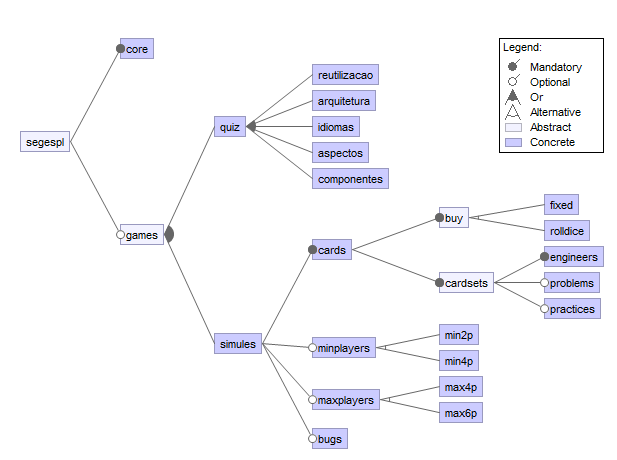
\includegraphics[width=0.8\textwidth]{img/features.png}
\caption{Modelo de Características}
\label{img:feature-model}
\end{figure}






\bibliographystyle{sbc}
\bibliography{bibfile}

\end{document}
